%!TeX root=Hauptdokument.tex
\chapter{Physikalische Grundlagen}

\section{Literatur -- Von Asimoov bis Kirk}

\blindtext[3]

\begin{center}
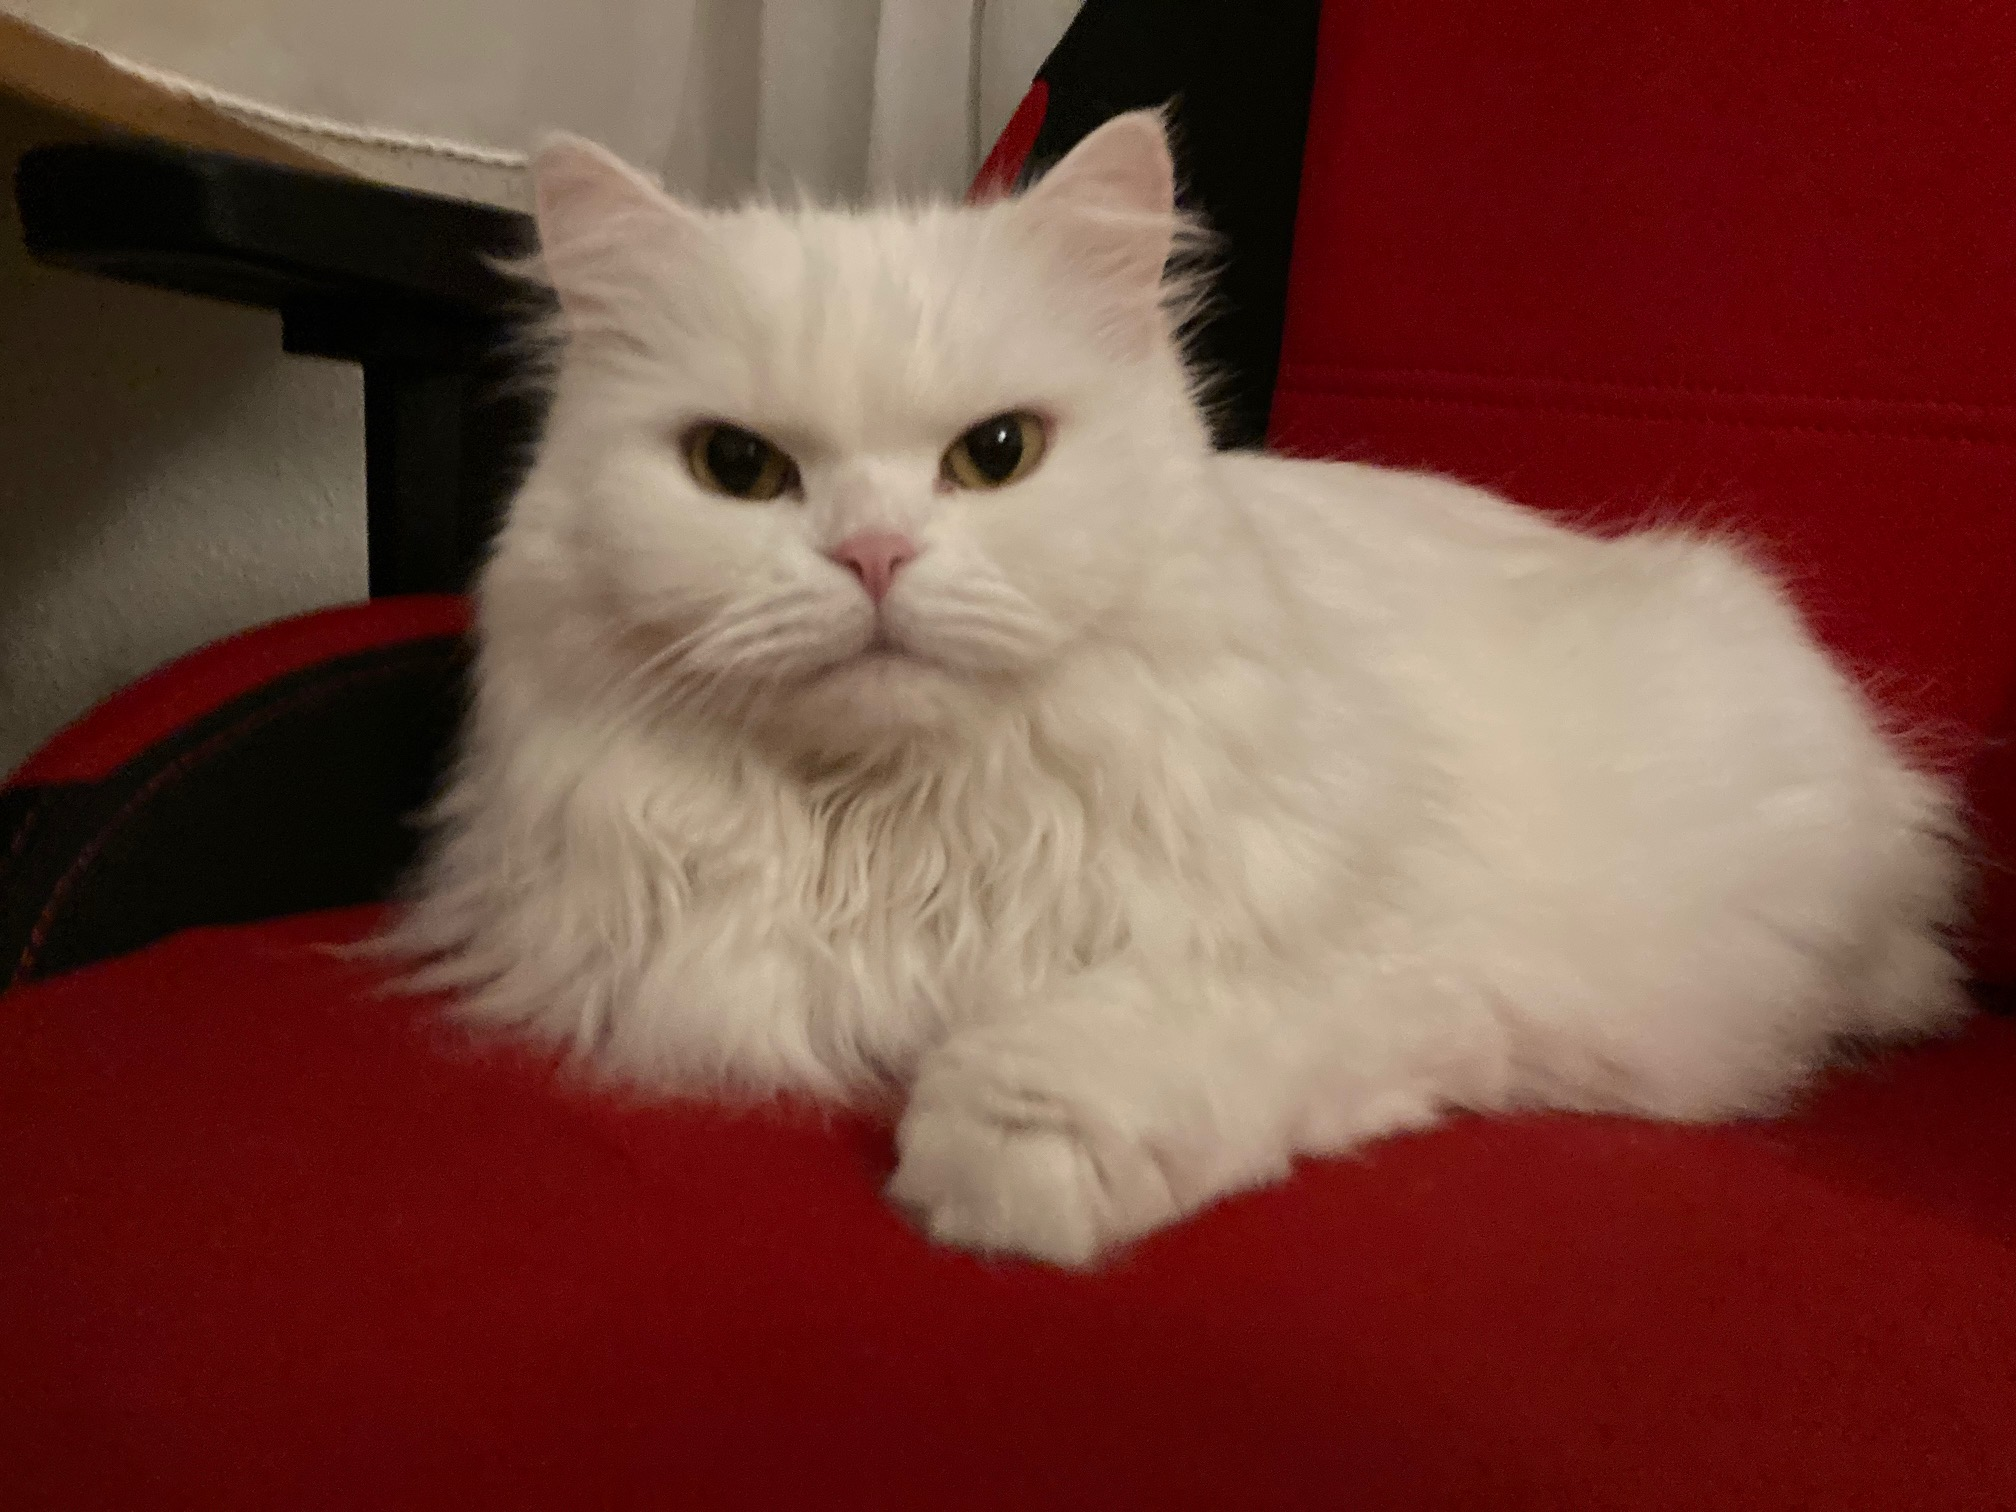
\includegraphics[width=0.8\textwidth]{Bilder/Katze.jpg}
\captionof{figure}{Meine Katze Melli}\label{fig:katze}
\end{center}


\blindtext[3]

\begin{figure}
\centering
\subcaptionbox{Eine Katze \label{cat1}}
{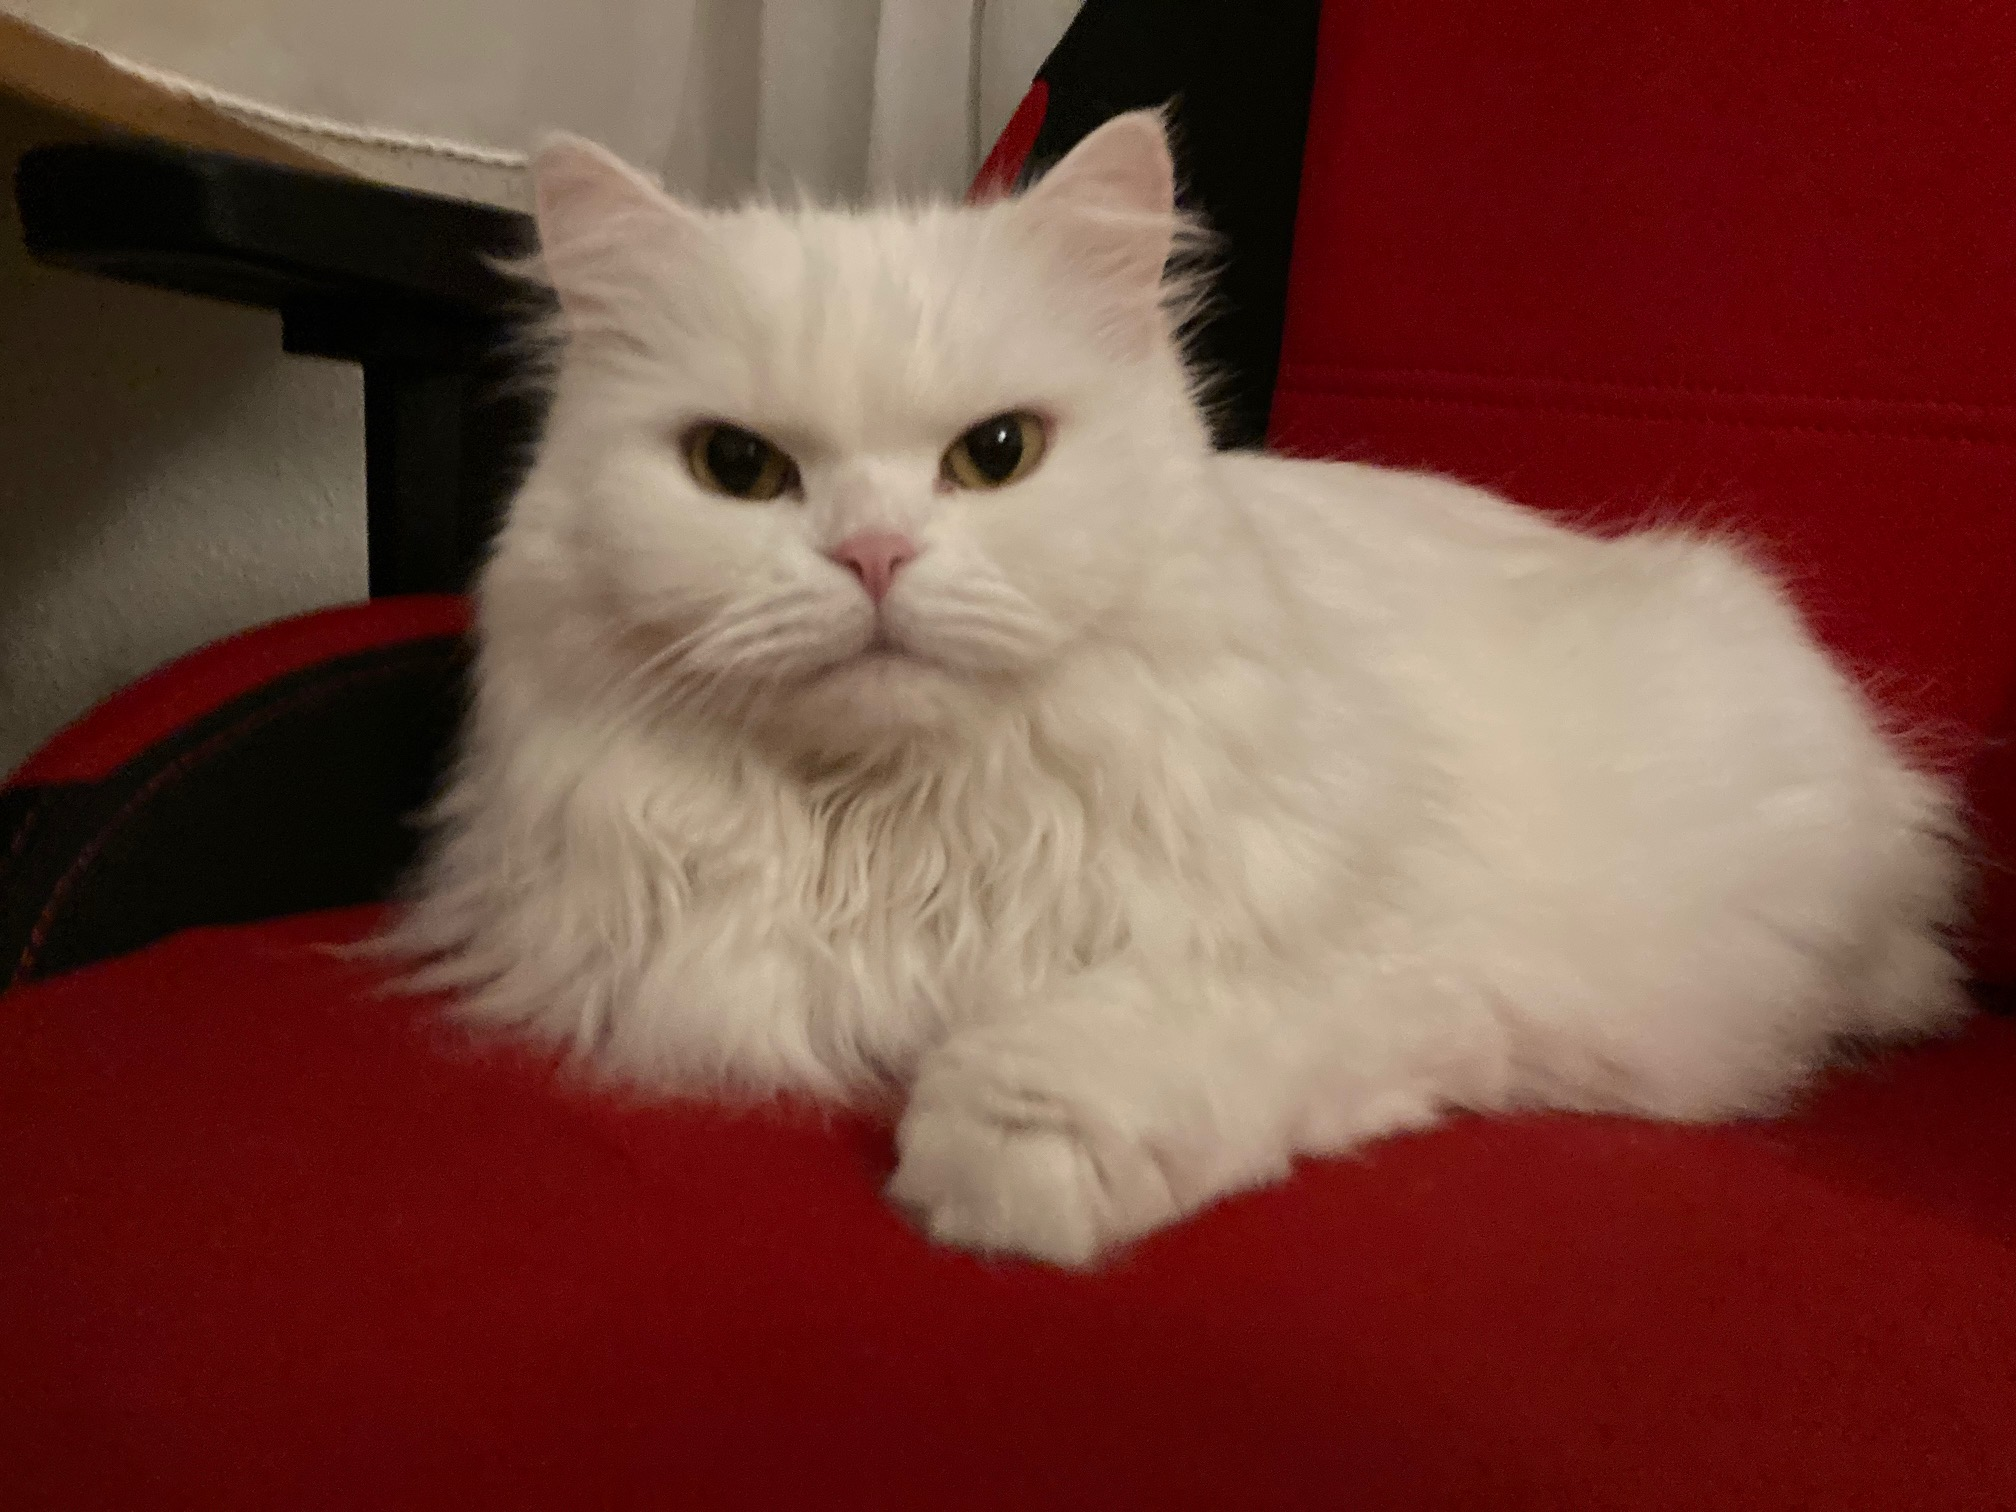
\includegraphics[width=0.49\textwidth]{Bilder/Katze}}
\subcaptionbox{Die selbe Katze \label{cat2}}
{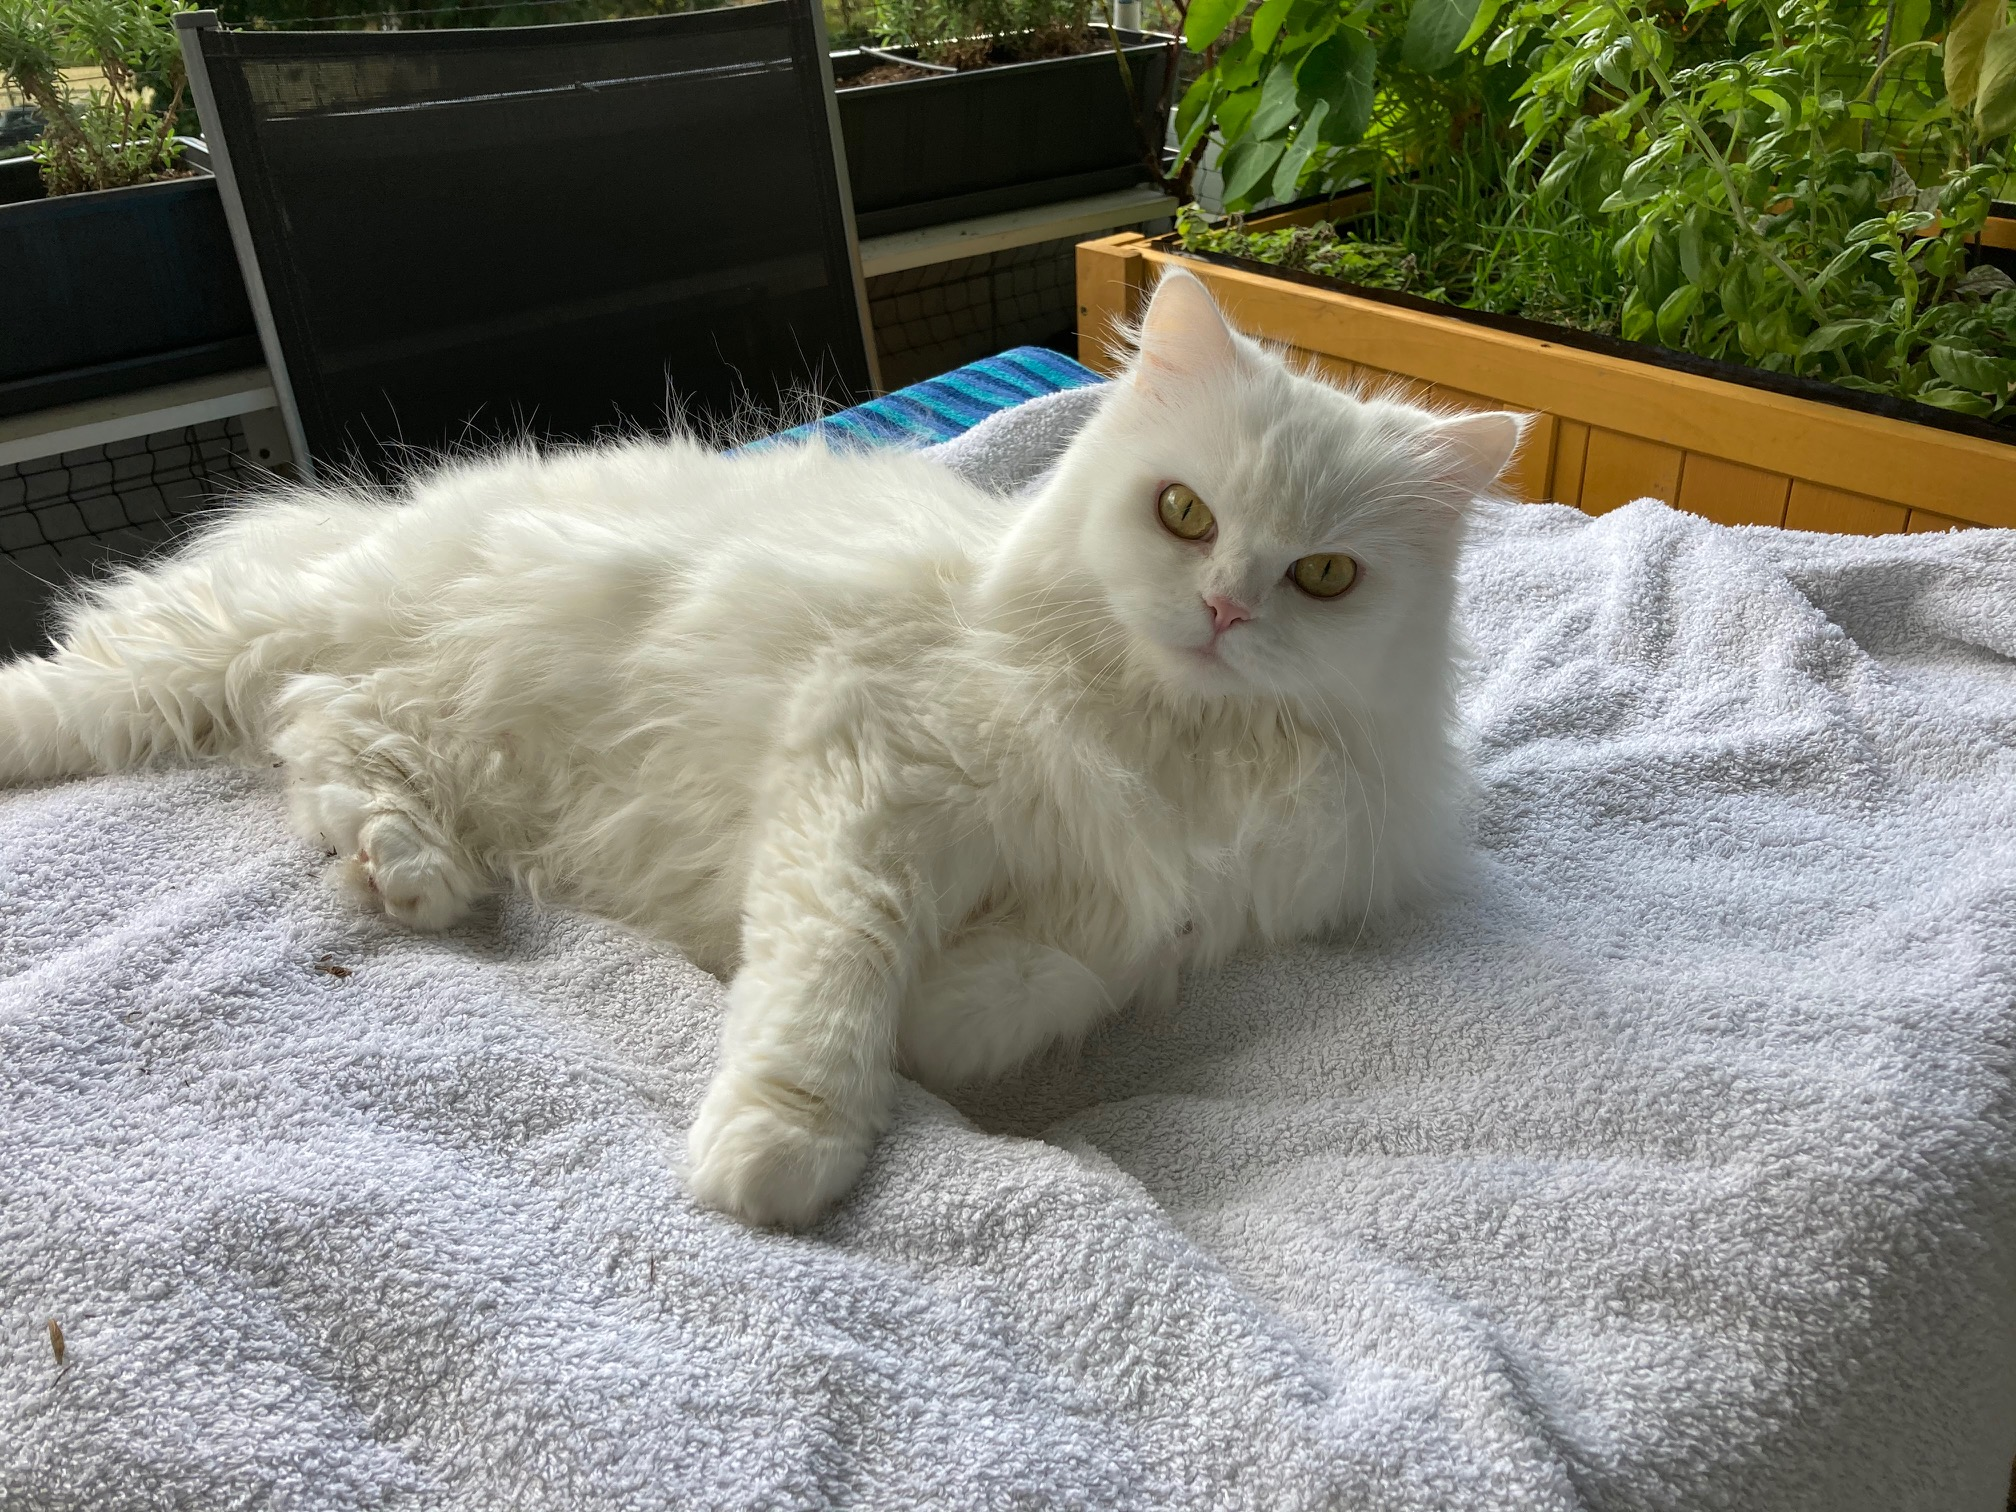
\includegraphics[width=0.49\textwidth]{Bilder/Katze1}}
%\caption{Zwei Katzenbilder}\label{katzenbilder}
\subcaptionbox{Eine Katze \label{cat1}}
{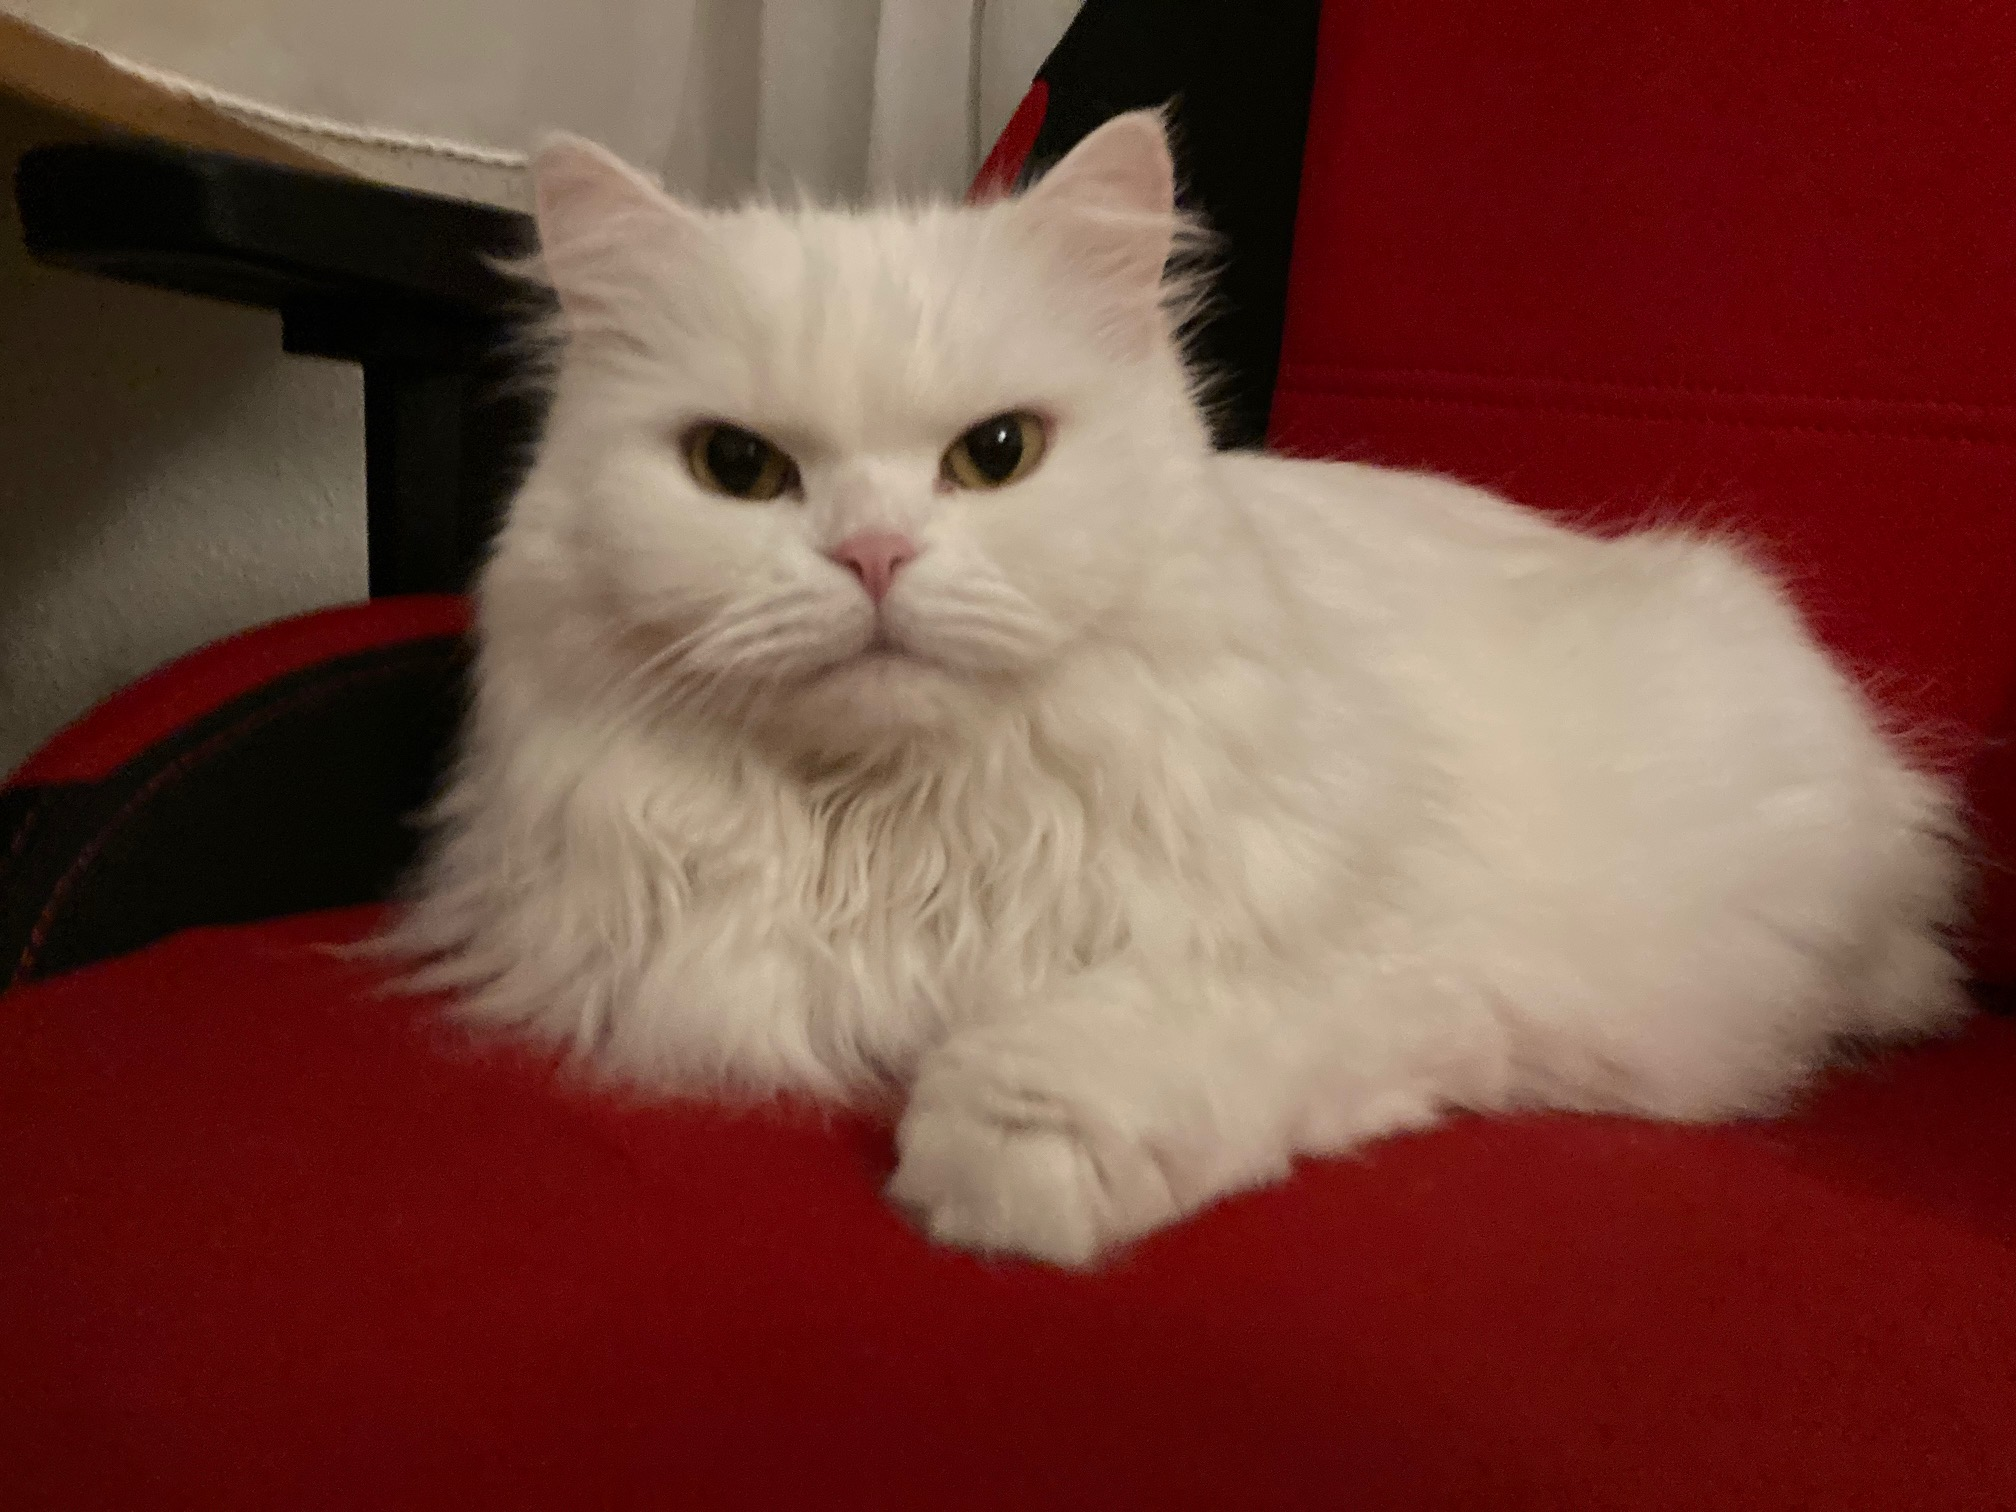
\includegraphics[width=0.49\textwidth]{Bilder/Katze}}
\subcaptionbox{Die selbe Katze \label{cat2}}
{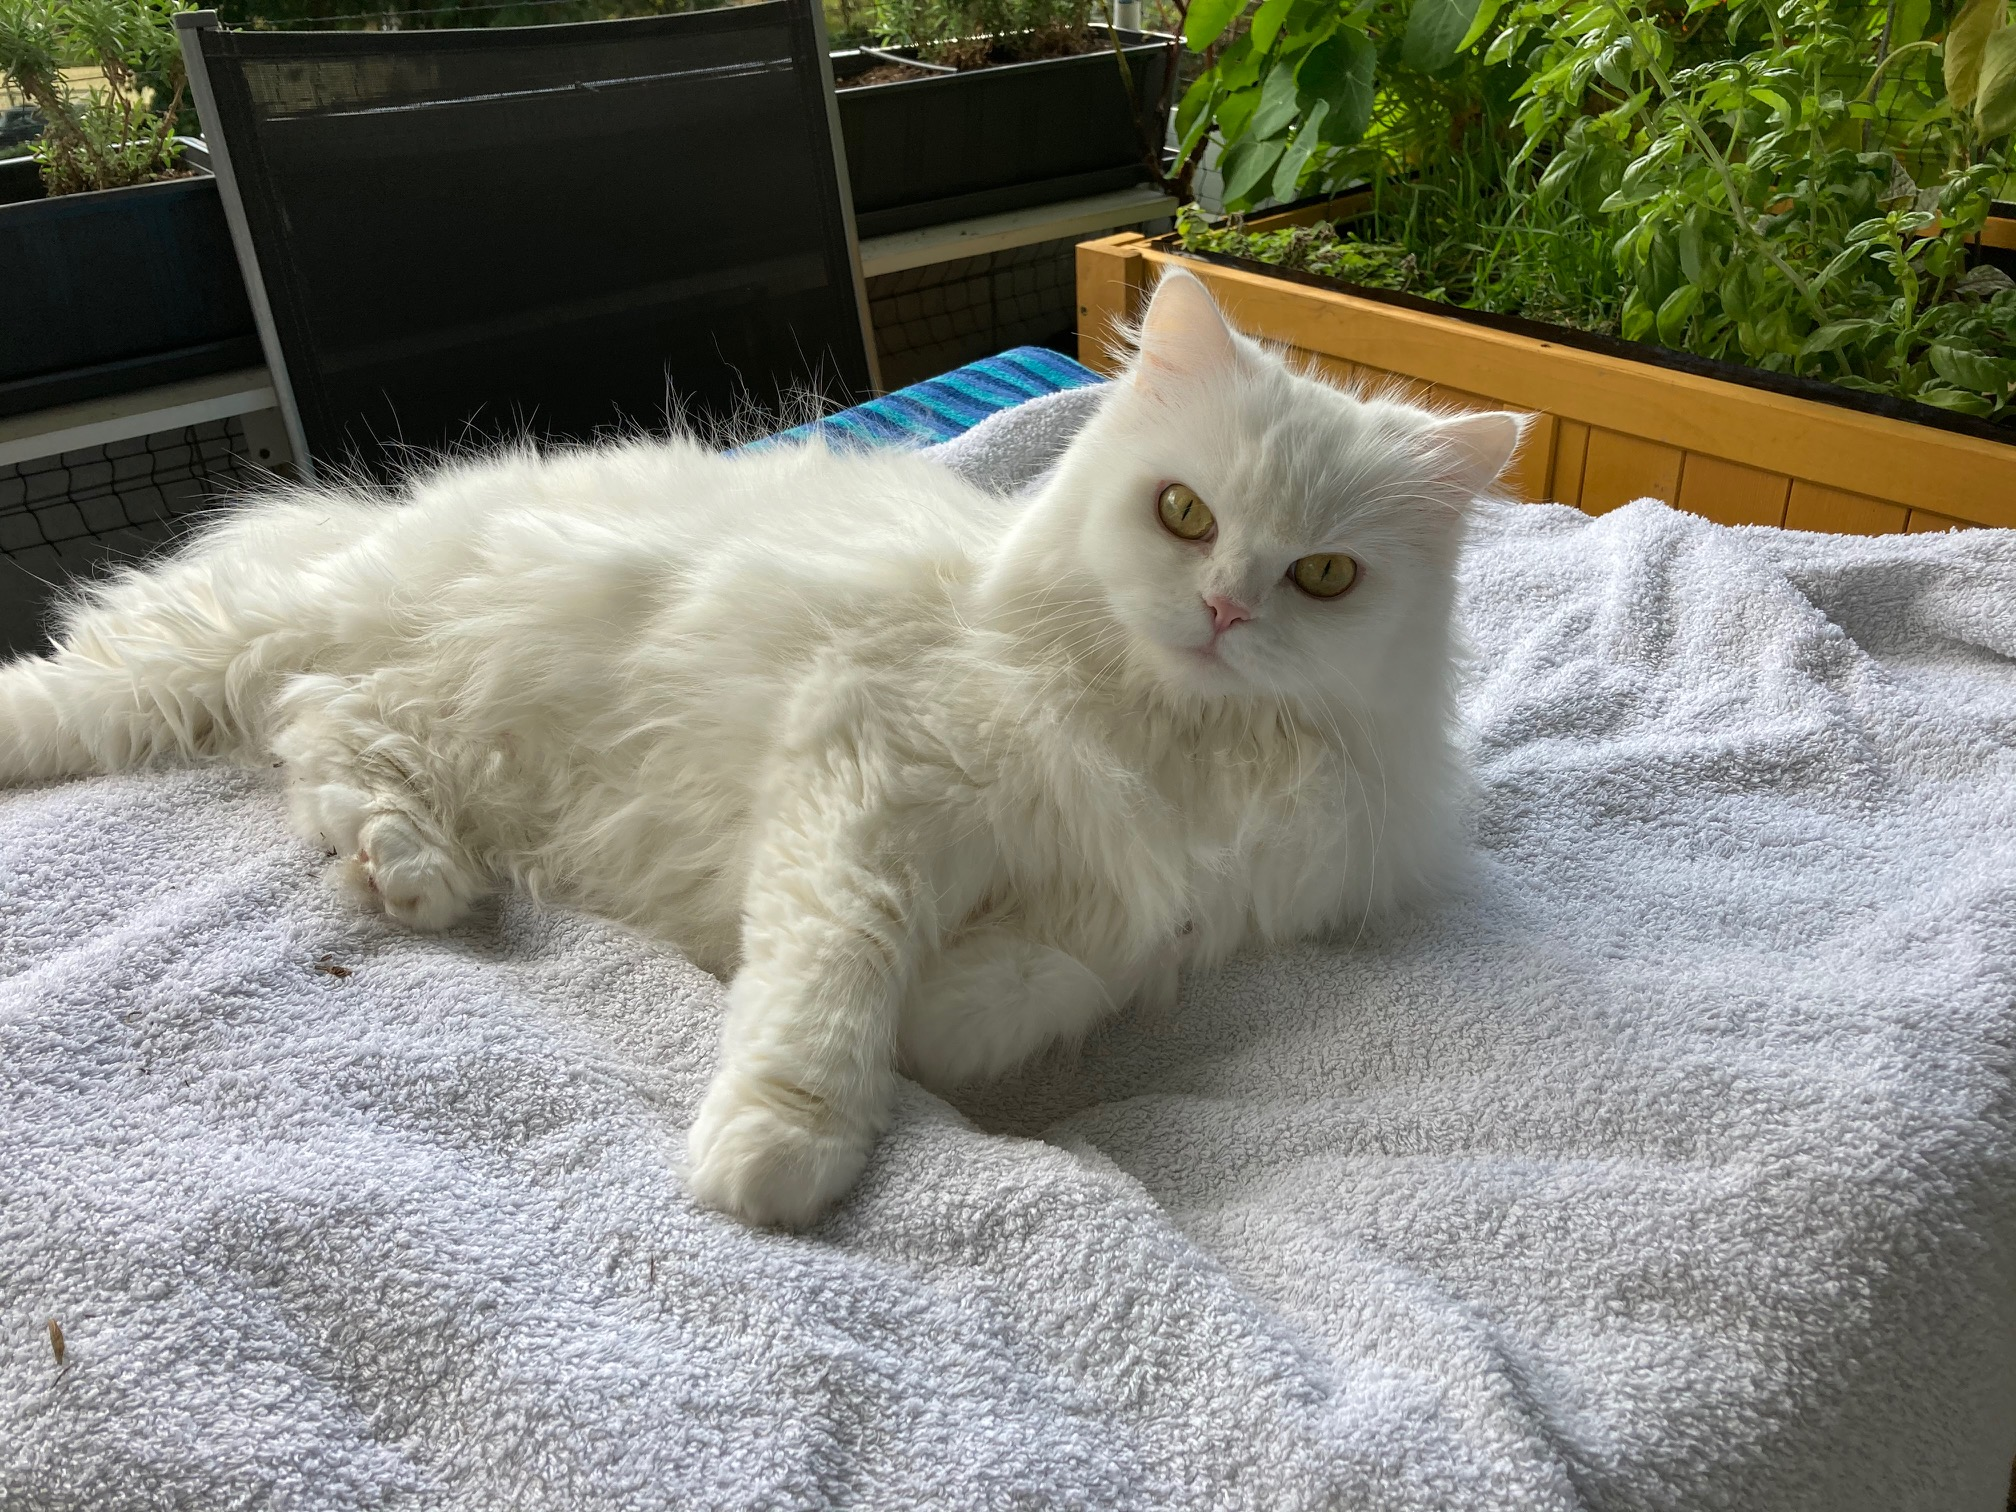
\includegraphics[width=0.49\textwidth]{Bilder/Katze1}}
\caption{Zwei Katzenbilder}\label{katzenbilder}
\end{figure}

Abbildung \ref{cat1} auf Seite \pageref{katzenbilder}

Abbildung \ref{cat2} auf Seite \pageref{katzenbilder}

Abbildung \ref{katzenbilder} auf Seite \pageref{katzenbilder}



\blindtext[3]

\blindtext[3]